\documentclass[letterpaper, 12pt]{article}

\usepackage{graphicx}
\usepackage{fancyhdr}
\usepackage[T1]{fontenc}
\usepackage{lmodern}
%\usepackage[francais]{babel}
\usepackage[frenchb]{babel}
\usepackage[applemac]{inputenc}
\usepackage{lipsum}
\usepackage{vmargin}
\usepackage{lastpage}
\usepackage{enumerate}
\usepackage{pdfpages}
\usepackage[nogin]{Sweave}
\usepackage{lscape}
\usepackage{color}
\usepackage{listings}
\usepackage{verbatim}
\usepackage{wrapfig}
\usepackage{hyperref}
\usepackage[all]{hypcap}

\usepackage{amssymb, amsmath}




\begin{document}

\begin{titlepage}
\vspace*{3cm}
\begin{center}

\huge{\bf Types of relation between \\ a variable and its probabilities}\\

\vspace*{2cm}
\large{By Benoit Bruneau}
\end{center}
\vspace*{4cm}

%\hangindent=1cm
%\begin{flushleft}
\begin{description}
\item[Package:] `bmisc'
\item[Version:] 0.2-12
\item[Depends:] car, lattice, zoo, robustbase, and methods
\item[Author \& Maintainer:] Benoit Bruneau (\href{mailto:benoit.bruneau1@gmail.com}{benoit.bruneau1@gmail.com})
\item[Description:] These functions can be used to estimate probabilities \verb=[0,1]= by specifying the inflection points of a relation. Described relations are of type `full', `ramp' and `logistic'.
\item[License:] LGPL $\geqslant$ 3.0
\end{description}


\vspace*{\fill;}


\end{titlepage}

\tableofcontents
\newpage

\section{Types `full' and `plat.full'}
\noindent These relations have "all-or-nothing" types of probabilities. One or two threshold (inflection points) need to be defined. 
The main difference between `full'(Figure~\ref{fig1}) and `plat.full' (Figure~\ref{fig2}) types 
are the number of thresholds. For all types, `plat' stands for "plateau".\\*

\begin{description}
\item[full.sel]\verb#(infl1, x, ptv=TRUE)#
\item[plat.full.sel]\verb#(infl1, infl2, x, ptv=TRUE)#
\end{description}
where \verb#infl1# and \verb#infl2# are the inflection points, \verb#x# is a numeric vector for which probabilities are 
estimated and \verb#ptv# indicates if the trend is positive  (\verb#TRUE#) or negative (\verb#FALSE#).\\*

Here are examples for these types:

\begin{Schunk}
\begin{Sinput}
> data = 0:3000
> full.sel(infl1 = 1500, x = data, ptv = TRUE)
> full.sel(infl1 = 1500, x = data, ptv = FALSE)
\end{Sinput}
\end{Schunk}
\begin{figure}[h]
\begin{center}
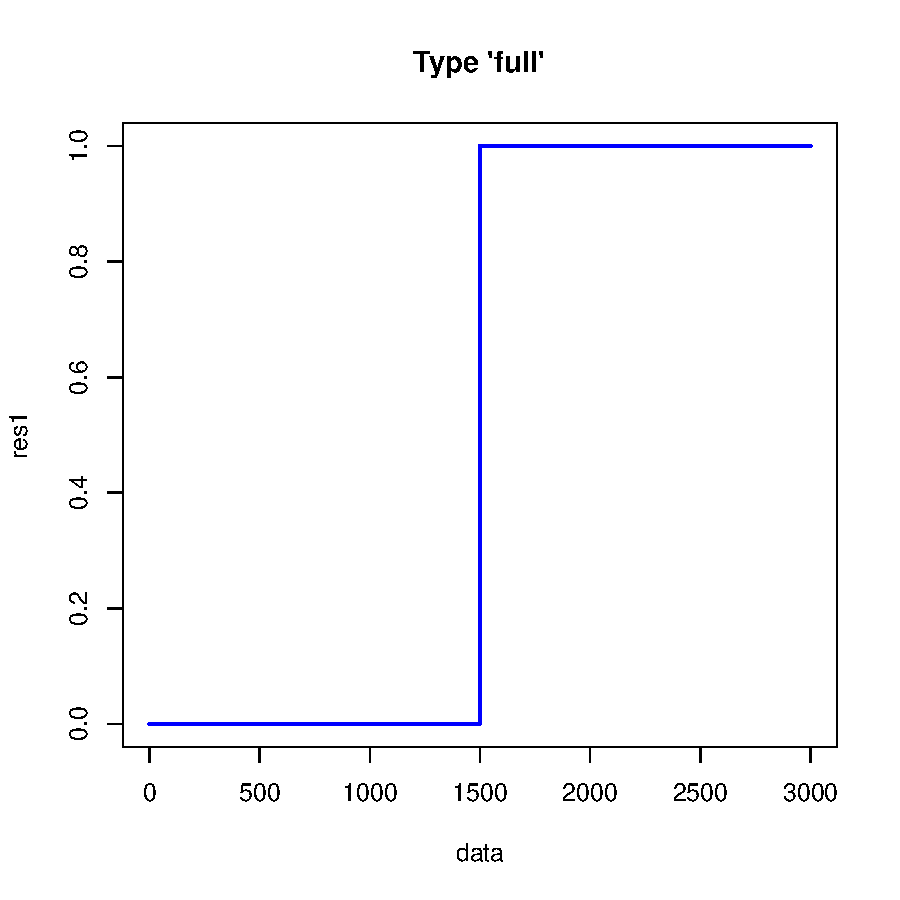
\includegraphics{relation_sel-002}
\end{center}
\caption{Type 'full' with pvt=TRUE in gray and pvt=FALSE in red.}
\label{fig1}
\end{figure}

\newpage
\begin{Schunk}
\begin{Sinput}
> data = 0:3000
> plat.full.sel(infl1 = 1000, infl2 = 2000, x = data, ptv = TRUE)
> plat.full.sel(infl1 = 1000, infl2 = 2000, x = data, ptv = FALSE)
\end{Sinput}
\end{Schunk}
\begin{figure}[h]
\begin{center}
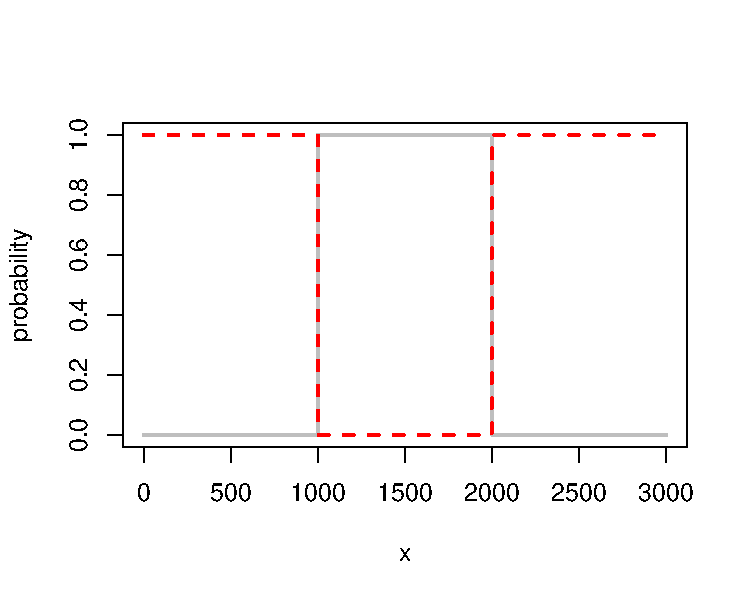
\includegraphics{relation_sel-004}
\end{center}
\caption{Type 'plat.full' with pvt=TRUE in gray and pvt=FALSE in red.}
\label{fig2}
\end{figure}


%%%%%%%%%%%%%%%%%%%%%%%%%%%%%%%%%%%%%%%%%%%%%%%%%%%%%%%%%%%%%%%%%%%%%%%%%%%%%%%%%%%%%%%%%%%%%%%%%%%
\newpage

\section{Types `ramp' and `plat.ramp'}
\noindent These relations involve adding a gradual increase (or decrease) of probabitily between two inflection points. 
They are an 'upgraded' version of `full' and `plat.full'. Two or four inflection points are needed. 
 The main difference between `ramp'(Figure \ref{fig3}) and `plat.ramp' (Figure \ref{fig4}) types are the number 
 inflection points.\\*

\begin{description}
\item[ramp.sel]\verb#(infl1, infl2, x, ptv=TRUE)#
\item[plat.ramp.sel]\verb#(infl1, infl2, infl3, infl4, x, ptv=TRUE)#
\end{description}
where \verb#infl1# to \verb#infl4# are the inflection points, \verb#x# is a numeric vector for which probabilities are 
estimated and \verb#ptv# indicates if the trend is positive  (\verb#TRUE#) or negative (\verb#FALSE#).\\*

Here are examples for these types:

\begin{Schunk}
\begin{Sinput}
> ramp.sel(infl1 = 1000, infl2 = 1500, x = data, ptv = TRUE)
> ramp.sel(infl1 = 1000, infl2 = 1500, x = data, ptv = FALSE)
\end{Sinput}
\end{Schunk}
\begin{figure}[h]
\begin{center}
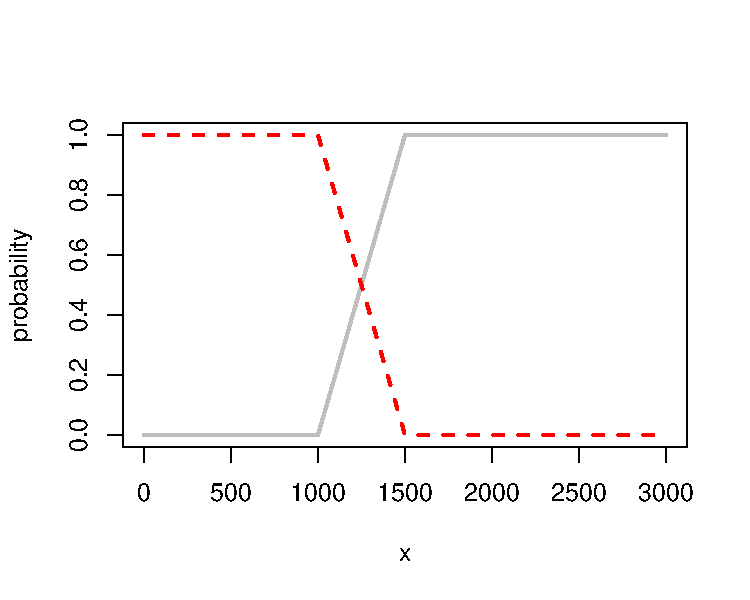
\includegraphics{relation_sel-006}
\end{center}
\caption{Type 'ramp' with pvt=TRUE in gray and pvt=FALSE in red.}
\label{fig3}
\end{figure}

\newpage
\begin{Schunk}
\begin{Sinput}
> data = 0:3000
> plat.ramp.sel(infl1 = 1000, infl2 = 1500, infl3 = 2000, infl4 = 2500, x = data, ptv = TRUE)
> plat.ramp.sel(infl1 = 1000, infl2 = 1500, infl3 = 2000, infl4 = 2500, x = data, ptv = FALSE)
\end{Sinput}
\end{Schunk}
\begin{figure}[h]
\begin{center}
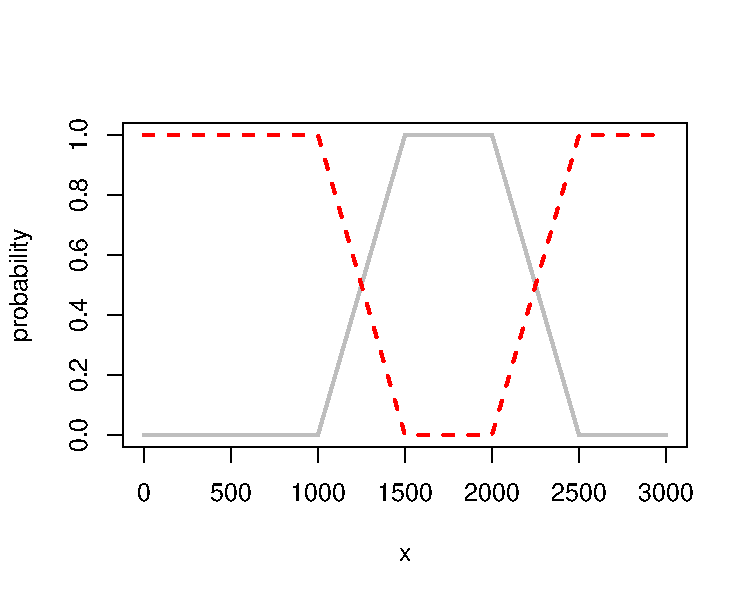
\includegraphics{relation_sel-008}
\end{center}
\caption{Type 'plat.ramp' with pvt=TRUE in gray and pvt=FALSE in red.}
\label{fig4}
\end{figure}





%%%%%%%%%%%%%%%%%%%%%%%%%%%%%%%%%%%%%%%%%%%%%%%%%%%%%%%%%%%%%%%%%%%%%%%%%%%%%%%%%%%%%%%%%%%%%%%%%%%
\newpage

\section{Types `logit' and `plat.logit'}
\noindent These relations use logistic curves. Inflection points are defined as points where the intantenuous splope 
is a proportion (\verb#prop#) of the intantenuous slope at $x_{50}$. These types make use of the function \verb#find.beta()# 
of \verb#package::bmisc#. Default value of \verb#prop# is \verb#0.1#. The end result is a logistic curve with 
$x_{50}$ being the midpoint between the inflection points. Two or four inflection points are needed. 
The main difference between `logit'(Figure \ref{fig5}) and `plat.logit' (Figure \ref{fig6}) types are the 
number inflection points.\\*
        
\begin{description}
\item[logit.sel]\verb#(infl1, infl2, x, ptv=TRUE)#
\item[plat.logit.sel]\verb#(infl1, infl2, infl3, infl4, x, ptv=TRUE)#
\end{description}
where \verb#infl1# to \verb#infl4# are the inflection points, \verb#x# is a numeric vector for which probabilities are 
estimated and \verb#ptv# indicates if the trend is positive  (\verb#TRUE#) or negative (\verb#FALSE#).\\*

Here are examples for these types:

\begin{Schunk}
\begin{Sinput}
> logit.sel(infl1 = 1000, infl2 = 1500, x = data, ptv = TRUE)
> logit.sel(infl1 = 1000, infl2 = 1500, x = data, ptv = FALSE)
\end{Sinput}
\end{Schunk}
\begin{figure}[h]
\begin{center}
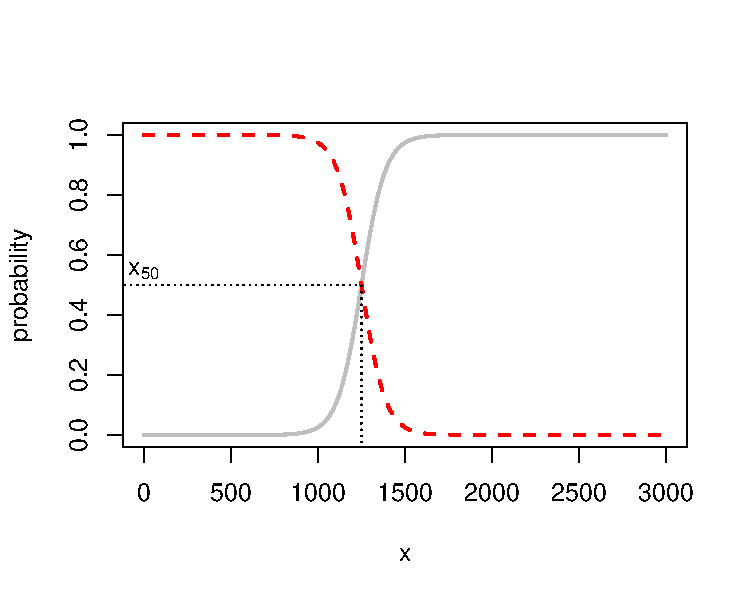
\includegraphics{relation_sel-010}
\end{center}
\caption{Type 'logit' with pvt=TRUE in gray and pvt=FALSE in red.}
\label{fig5}
\end{figure}

\newpage
\begin{Schunk}
\begin{Sinput}
> data = 0:3000
> plat.logit.sel(infl1 = 1000, infl2 = 1500, infl3 = 2000, infl4 = 2500, x = data, ptv = TRUE)
> plat.logit.sel(infl1 = 1000, infl2 = 1500, infl3 = 2000, infl4 = 2500, x = data, ptv = FALSE)
\end{Sinput}
\end{Schunk}
\begin{figure}[h]
\begin{center}
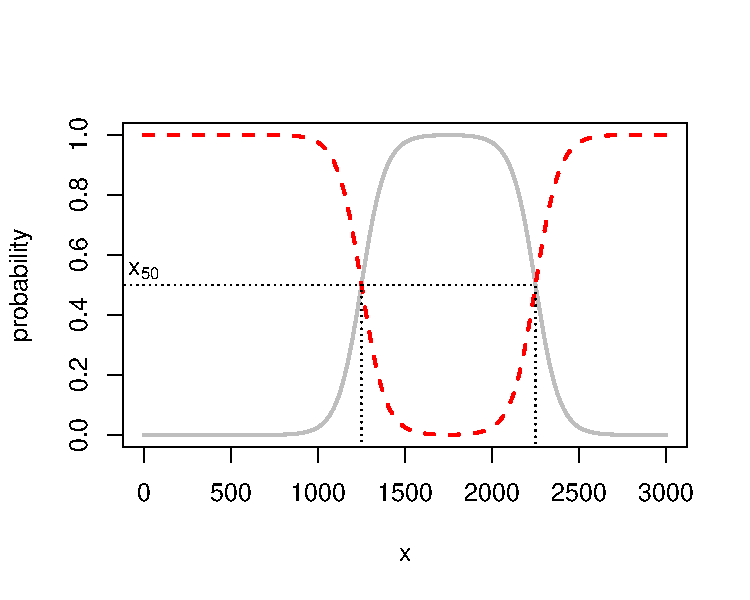
\includegraphics{relation_sel-012}
\end{center}
\caption{Type 'plat.logit' with pvt=TRUE in gray and pvt=FALSE in red.}
\label{fig6}
\end{figure}

        
        
        
        
        
\end{document}
